\documentclass[../main.tex]{subfiles}
\begin{document}

\chapter{Lecture 22 - 26-05-2020}

\section{Continous of Pegasos}
$$
w_s = arg \min (\hat{\ell}_s(w) + \frac{\lambda}{2} \|w\|^2 
\qquad \frac{(2 \, L )^2}{\lambda \, m}-stable
$$
$$
\ell(w, (x,y)) = \left[ 1 - y w^T x \right]_+
$$
\begin{figure}[h]
    \centering
    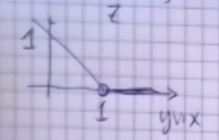
\includegraphics[width=0.3\linewidth]{../img/lez22-img1.JPG}
    \caption{}
    %\label{fig:}
\end{figure}
$$
\nabla \ell(w, (x,y)) = - y x I \{ w^T \, x \leq 1 \} \qquad \| \nabla \ell(w,z) \| \leq \|x \| \leq X
$$
$$
\ell(w,z) - \ell(w,z) \leq \nabla \ell(w',z)^T (w-w') \leq \| \red{ \nabla \ell(w',z) \| } \| w-w'\|
$$
where \bred{red} is equal to $X$
$$
\hat{\ell}_s(w_s) \leq \hat{\ell}(w_s) + \frac{1}{2} \|w_s \|^2 \leq \hat{\ell}_s(u) + \frac{1}{2} \| u \|^2 \qquad \forall u \in \barra{R}^d
$$
$$
E [ \ell_D(w_s)] \leq  E[ \hat{\ell}(w_s)] + \frac{4 \, x^2}{\lambda \, m} \leq E [ \hat{\ell}_s(u) + \frac{1}{2} \|u\|^2 ] + \frac{4 \, X^2}{\lambda \, m} =
$$
$$
= \ell_D(u) + \frac{\lambda}{2} \| u \|^2 + \frac{4 \, x^2}{\lambda \, m}
$$

$$
E [ \ell_D(w_s) ] \leq min( \ell_D(u) + \frac{\lambda}{2}
\| u\|^2) +\frac{4 \, x^2}{\lambda \, m} $$

$$
\ell_D^{0-1}(w_s) \leq \ell_D(w_s)
$$
$$
0-1 \ loss \ \leq \ hinge
$$

$$
E [ \ell_D(w_s) ] + \ell_D(u) + \frac{\lambda}{2} \|u \|^2 + \frac{4 \, x^2}{\lambda \, m } \qquad \lambda \approx \frac{1}{\sqrt[]{m}}
$$
\\
We can run SVM in a Kernel space $H_k$:
$$
g_s = arg \min_{g \in H_k} (\hat{\ell}_s(g) - \frac{\lambda}{2} \|g\|^2 k )  
$$
$$
g = \sum_{i = 1}^N \alpha_i \, k (x_i, \cdot) \qquad h_t(g) = [ 1-y_t g(x_t) ]_+
$$
\\
If $H_k$ is the kernel space induced by the Gaussian Kernel, then elements of $g$ can approximate any continous function $\Rightarrow$ \bred{ consistency}
\\
SVM with Gaussian Kernel is consistent if $\lambda = \lambda_m $ \qquad (with $0$-$1$ loss)
\\
1) $\lambda_m = o(\lambda)$\\
2) $\lambda_m = w (m^{-\frac{1}{2}}) $
\\
$$
\lambda_m \approx \frac{\ln m}{\sqrt[]{m}} \quad  \surd
$$\\
\section{Boosting and ensemble predictors }
Examples:
\begin{itemize}
\item Stochastic gradiant descent (SGD)
\end{itemize}
$A \qquad h_1, ..., h_T$ \ Given $S$, example from $S$: $_1,...,S_T$
\\
$h_1 = A(S_1)$ \ is the output 1
\\
Assume we are doing binary classification with $0$-$1$ $loss$.
\\
$
h_1,...,h_T : X \rightarrow \{-1,1\}
$ \qquad (We go for a majority vote classifier)
\\
$
x \quad h_1(x),...,h_T(x) \in \{-1,1\} \qquad f = sgn \left( \sum_{t=1}^T h_t \right)
$
\\
Ideal condition $Z$ is the index of a training example from $S$ drawn at random (uniformly):
$$
P \left(h_1(x_2) \neq y_z \wedge ... \wedge h_t(x_z) \neq y_z \right) = \prod_{i=1}^T P\left(h_i(x_z) \neq y_z \right)
$$
The error probability of each $h_i$ is independent from the others.
\\
Define the training error of the classifier:
$$
\hat{\ell}_s(h_i) = \frac{1}{m} \sum_{t=1}^m I \{h_t(x_t) \neq y_t \} = P \left(h_t(x_z) \neq y_z \right)
$$

We can assume $\hat{\ell}_s(h_i) \leq \frac{1}{2} \quad \forall i = 1,...,T$
\\
(Take $h_i$ or any $h_T$)
\\\\
I want to bound my majority vote $f$
$$
\hat{\ell}_s(f) = P \left( f(x_z) \neq y_z \right) = P\left( \sum_{i=1}^T I \{h_i(x_z) \neq y_z \} > \frac{T}{2} \right)
$$
If half of them are wrong
$$
\hat{\ell}_{ave} = \frac{1}{T} \sum_{i=1}^T \hat{\ell}_s(h_t) \ = \ P \left( \frac{1}{T} \sum_{i=1}^T I \{ h_i(x_z) \neq y_z \} > \hat{\ell}_{ave} + \left( \frac{1}{2} -\hat{\ell}_ave\right) \right)
$$
$ B_1, ..., B_T \quad B_1 = I \{ h_i (x_z) \neq y_z \}$
\\
And because of our independence assumption, we know that $B_1,..,B_T$ are independent
\\
$$
E\left[ B_i \right] = \hat{\ell}_s(h_i)
$$
We can apply Chernoff-Hoffding bounds to $B_1,...,B_t$ even if they don't have the same expectations
$$
P \left( \frac{1}{T} \sum_{i=1}^T B_i > \hat{\ell}_ave + \varepsilon \right) \leq e^{-2 \, \varepsilon^2 \, T} \qquad \varepsilon = \frac{1}{2} - \hat{\ell}_{ave} \geq 0
$$
$$
P(f(x_z) \neq y_z) \leq e^{-2 \, \varepsilon^2 \, T}
\qquad
\gamma_i = \frac{1}{2} - \hat{\ell}_s(h_i) \quad \frac{1}{T} \sum_i \gamma_i = \frac{1}{2} - \hat{\ell}_{ave} 
$$
$$
\hat{\ell}(f) \leq \exp\left(-2 T \left( \frac{1}{T} \sum_i \gamma_i \right)^2\right)
$$
\\ 
where $\gamma_i$ is the edge of $h_i$
\\
If $\gamma_i \geq \gamma \forall i = 1,...,T$, then the training error of my majority vote is: $$\hat{\ell}(f) \leq e^{-2 \, T \, \gamma^2}$$
How do we get independence of $h_i(x_z) \neq y_z$?
\\
We can't guarantee this!
\\
The subsampling of $S$ is attempting to achieve this independence.

\newpage
\subsection{Bagging}
It is a meta algorithm!
\\
$S_i$ is a random (with replacement) subsample of $S$ of size $|s_i| = |S|$.
\\ So the subsample have the same size of the initial training.
\\
$$| S_i  \nabla S| \qquad |S_i \cap S | \leq \frac{2}{3}$$
$N = $ \# of unique points in $S_i$ (did non draw them twice from $S$)
\\
$x_t = I \{ (x_t,y_t)$ is drawn in $S_i \}$ \qquad $P(x_t = 0 ) = (1- \frac{1}{m})$
$$
E [N] = \sum_{t=1}^m P(x_t=1)
\ = \ \sum_{t=1}^m (1 - (1-\frac{1}{m})^m) 
\ = \  m -m (1-\frac{1}{m})^m
$$
Fraction of unique points in $S :$
$$ \frac{E[N]}{m} = 1-(1- \frac{1}{m})^m =_{m \rightarrow \infty} 1-e^{-1} \approx 0,63$$
So $\frac{1}{3}$ will be missing.
\\
\subsection{Random Forest}
Independence of errors helps bias.\\ randomisation of subsampling helps variance.
\begin{itemize}
\item 1) Bagging over Tree classifiers (predictors)
\item 2) Subsample of features\\
\end{itemize}
\begin{figure}[h]
    \centering
    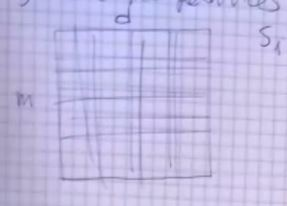
\includegraphics[width=0.3\linewidth]{../img/lez22-img2.JPG}
    \caption{}
    %\label{fig:}
\end{figure}
Control $H$ of subsample features depth of each tree.
\\Random forest is typically good on many learning tasks.
\\
Boosting is more recent than bagging and builds independent classifiers "by design". 
$$ \hat{\ell}(f) \leq e^{-2 \, T \gamma^2} \qquad \gamma_i> \gamma$$
$$ \gamma_i = \frac{1}{2}-\hat{\ell}_s(h_i) \quad \textit{edge of $h_i$}
$$
where $ \hat{\ell}_s(h_i)$ is weighted training error
\end{document}